\documentclass{article}
\usepackage{/Users/jay/LaTeX/cs}
\usepackage{/Users/jay/LaTeX/matlab}

\newcommand{\hmwkClass}{Digital Image Processing, Spring 2018}
\newcommand{\hmwkTitle}{Homework 3}
\newcommand{\hmwkDueDate}{May 2, 2018}
\newcommand{\tb}{\textbf}

\begin{document}

\thispagestyle{empty}
\section*{\hmwkClass \\
    \normalsize{\hmwkTitle} \\
    \normalsize{DUE DATE: \hmwkDueDate}
}

\hfill{Student ID: B03902129 \, Department: CSIE \, Name: Peng-Yu Chen}

% ------ %
% README %
% ------ %
\subsection*{README}

To run my program, simply type \tb{README} in the Command Window of MATLAB application, then it'll run all .m files and output the .raw images.

\begin{lstlisting}[caption = {README.m}]
    % DIP Homework Assignment #3 
    % May 2, 2018
    % Name: Jay Chen
    % ID #: B03902129 
    % email: b03902129@ntu.edu.tw
    
    %#########################################################################
    % Add path first
    %#########################################################################
    
    disp('Add path "./prob1", "./prob2", "./bonus" and "./readwriter"');
    addpath('./prob1');
    addpath('./prob2');
    addpath('./bonus');
    addpath('./readwriter');
    
    disp('Make a parent folder "./outputs"');
    mkdir . outputs
    
    %######################################################################### 
    % Problem 1: MORPHOLOGICAL PROCESSING                                           
    % Implementation 1: Boundary extraction, I1 -> B     
    % Implementation 2: Count the number of objects based on morphological
    %                   processing
    % Implementation 3: Skeletonizing, I1 -> S
    % M-files: prob1.m, boundaryExtract.m, countObjects.m, dilateBinary.m, 
    %                   label.m and skeletonize.m
    % Output: B.raw and S.raw
    % Usage: run prob1 to call other .m files
    % Parameters:
    %       * Boundary Extraction: window size = 3 x 3
    %       * Dilation: window size = 9 x 9
    %       * Skeletonizing: 8-neighbors
    %#########################################################################
    
    fprintf('----------------------------------------\n');
    fprintf('Running "prob1"\n----------------------------------------\n');
    prob1();
    
    %######################################################################### 
    % Problem 2: TEXTURE ANALYSIS                                           
    % Implementation 1: Perform Law's method, I2 -> K         
    % Implementation 2: Generate another texture image, K -> exchanged
    % M-files: prob2.m, law.m, computeEnergy.m, kmeans.m, findTextures.m, 
    %          crossMedianFilter.m and exchange.m
    % Usage: run prob2 to call other .m files
    % Output: K.raw
    % Parameters:
    %       * Energy Computation: window size = 13
    %       * kmeans: initial centroids: (128, 128), (256, 256) and (384, 384)
    %       * Texture finding: 
    %           * T1(i, j) = 13520
    %           * T1(i, j) > 20000 && T2(i, j) > 3500
    %       * Cross Median Filter: window size = 61
    %#########################################################################
    
    fprintf('----------------------------------------\n');
    fprintf('Running "prob2"\n----------------------------------------\n');
    prob2();
    
    %######################################################################### 
    % Bonus                                           
    % Implementation 1: Produce an image by appropriate morphological
    %                   processing
    % M-files: bonus.m and dilate.m
    % Usage: run bonus to call other .m files
    % Output: None
    % Parameters:
    %       * Cross Median Filter: window size = 25
    %       * Dilation: window size = 11
    %#########################################################################
    
    fprintf('----------------------------------------\n');
    fprintf('Running "bonus"\n----------------------------------------\n');
    bonus();      
\end{lstlisting}

\newpage
% ----------------------------------- %
% PROBLEM 1: Morphological Processing %
% ----------------------------------- %
\subsection*{PROBLEM 1: Morphological Processing}

    Given a binary image $I_1$ as shown in Fig. 1. White pixels represent the objects and black pixels represent the background. Please follow the instructions below to create several new images and describe the method in detail for each case.

    \begin{enumerate}[label=(\alph*)]
        \item Perform boundary extraction on $I_1$ to extract the objects' boundaries and output the result as image $B$. Please provide some discussions about image $B$.

        I perform boundary extraction by the following formula:

        $$B(I_1(j, k)) = I_1(j, k) - (I_1(j, k) \ominus H(j, k)).$$

        \begin{enumerate}[label=(\roman*)]
            \item Calculate $(I_1(j, k) \ominus H(j, k))$.

                Initialize a zeros array $I_1H$ to denote $(I_1(j, k) \ominus H(j, k))$ first.
                
                For each point, we create a $3 \times 3$ window, if there isn't any $0$ in the window, we turn the $I_1H(j, k)$ to be 255 (white); otherwise, it remains 0 (black).

            \item Calculate $B(I_1(j, k)) = I_1(j, k) - (I_1(j, k) \ominus H(j, k))$ directly.
        \end{enumerate}

        \begin{figure}[!htb]
            \centering
            \begin{subfigure}[b]{0.3\textwidth}
                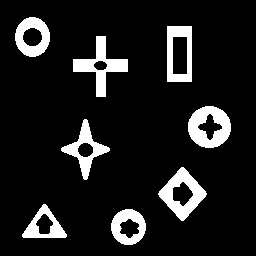
\includegraphics[width=\textwidth]{img/I1.png}
                \caption{I1.raw}
            \end{subfigure}
            ~
            \begin{subfigure}[b]{0.3\textwidth}
                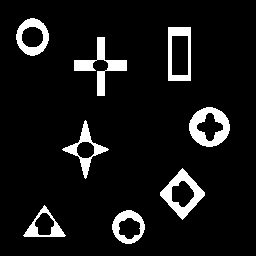
\includegraphics[width=\textwidth]{img/I1H.png}
                \caption{$I_1 \ominus H$}
            \end{subfigure}
            ~
            \begin{subfigure}[b]{0.3\textwidth}
                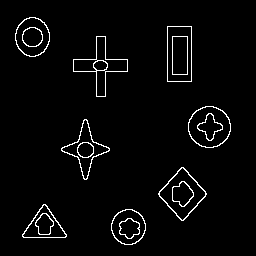
\includegraphics[width=\textwidth]{img/B.png}
                \caption{B.raw}
            \end{subfigure}

            \caption{Boundary Extraction}
        \end{figure}

        \item Please design an algorithm to count the number of objects in $I_1$ based on morphological processing.

        \begin{enumerate}[label=(\roman*)]
            \item To find the number of objects, I notice that there are some spaces in the objects, so I perform \textit{dilation} with a $9 \times 9$ structure element with $1$s first.

            $$Dilated(j, k) = I_1(j, k) \oplus H(j, k)$$

            \item After perform dilation, we initialize an array $Labeled$ with zeros and a variable $labelNum = 1$.
        
            \item For each entry, we labeled the $Labeled$ array with 4-connectivity by depth first search.
        
            \begin{lstlisting}
    if Dilated(i, j) == 1 && Labeled(i, j) == 0
        Labeled(i, j) = labelNum;
        Labeled = label(Dilated, Labeled, labelNum, i, j, h, w);
        labelNum = labelNum + 1;
    end
            \end{lstlisting}

            \newpage
            There are four cases:

            \begin{enumerate}
                \item $Dilated(i + 1, j) == 1$ and $L(i + 1, j) == 0$
                \item $Dilated(i - 1, j) == 1$ and $L(i - 1, j) == 0$
                \item $Dilated(i, j + 1) == 1$ and $L(i, j + 1) == 0$
                \item $Dilated(i, j - 1) == 1$ and $L(i, j - 1) == 0$
            \end{enumerate}

            Each case will recursively call the $label$ function with the same orientation.
            
            The program will finally output the $max(Labeled) = 8$.
        \end{enumerate}

        \begin{figure}[!htb]
            \centering
            \begin{subfigure}[b]{0.3\textwidth}
                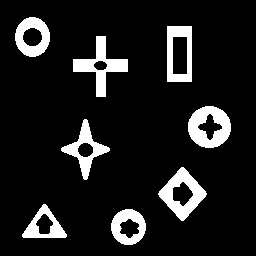
\includegraphics[width=\textwidth]{img/I1.png}
                \caption{I1.raw}
            \end{subfigure}
            ~
            \begin{subfigure}[b]{0.3\textwidth}
                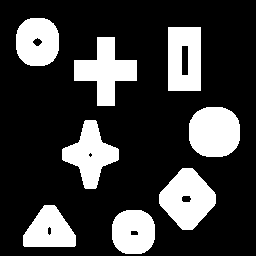
\includegraphics[width=\textwidth]{img/Dilated.png}
                \caption{$Dilated$}
            \end{subfigure}
            ~
            \begin{subfigure}[b]{0.3\textwidth}
                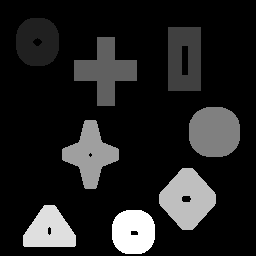
\includegraphics[width=\textwidth]{img/Labeled.png}
                \caption{$Labeled$ by different intensities}
            \end{subfigure}

            \caption{Count Objects and Label}
        \end{figure}

        \item Perform skeletonizing on $I_1$ and output the result as image $S$. Please provide some discussions about image $S$. \\

        Here I implement the \href{https://blog.csdn.net/zhubaohua_bupt/article/details/76850555}{Zhang Suen Thinning Algorithm} found in the web.

        \begin{enumerate}[label=(\roman*)]
            \item Convert the $I_1$ to $logical(I_1)$ array with only $0$s and $1$s.
            \item Initialize variables $isChange = true$ and an array $deletion$ with $1$s.
            \item While $isChange == true$, we first set the $isChange = false$, then we determine the $deletion$ array in two steps for each while-loop.
                    
            \item For each entry, we let $P$ equals to the element of $I_1(j, k)$ + its 8 neighbors (clockwise from $I_1(j - 1, k)$) and we calculate the boolean variable $cond$ based on which step we take:
            \begin{lstlisting}
    if step == 1
        cond = (S(i, j) == 1 && sum(P(2: end - 1)) <= 6 && sum(P(2: end - 1)) >=2 && P(2) * P(4) * P(6) == 0 && P(4) * P(6) * P(8) == 0);
    elseif step == 2
        cond = (S(i, j) == 1 && sum(P(2: end - 1)) <= 6 && sum(P(2: end - 1)) >=2 && P(2) * P(4) * P(8) == 0 && P(2) * P(6) * P(8) == 0);
    end
            \end{lstlisting}
                        
            \item We then determine the $deletion$ array by
            
            \begin{lstlisting}
    if cond
        A = 0;
        for k = 2: size(P, 2) - 1
            if P(k) == 0 && P(k + 1) == 1
                A = A + 1;
            end
        end
        if A == 1
            deletion(i, j) = 0;
            isChange = true;
        end
    end
        \end{lstlisting}
        \end{enumerate}

        \begin{figure}[!htb]
            \centering
            \begin{subfigure}[b]{0.3\textwidth}
                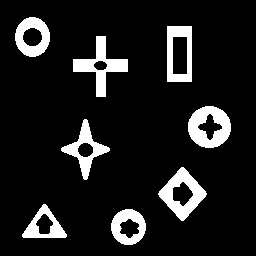
\includegraphics[width=\textwidth]{img/I1.png}
                \caption{I1.raw}
            \end{subfigure}
            ~
            \begin{subfigure}[b]{0.3\textwidth}
                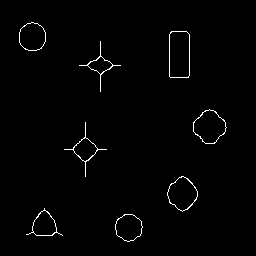
\includegraphics[width=\textwidth]{img/S.png}
                \caption{S.raw}
            \end{subfigure}

            \caption{Count Objects and Label}
        \end{figure}

        The algorithm is to thin the input image $I_1$ until there is no change. I calculate the skeletonized image with 8-neighbors. The skeletonized image is a thinnest image without changing the topological order but it'll sacrifice some details of the original image.

    \end{enumerate}

\newpage
\subsection*{PROBLEM 2: Texture Analysis}
    An image $I_2$ which is composed of several different textures is given in Fig. 2.

    \begin{enumerate}[label=(\alph*)]
        \item Perform Law's method on $I_2$ to segment the image into 3 different texture groups. Label the pixels of the same texture group with the same intensity values. Please detail the method you choose, specify all the parameters and output the result as $K$.
        
        After performing Law's method on $I_2$, we'll obtain
        
        $$M_i = I_2 \otimes H_i, \text{where $H_i$ is laws' masks and } i = 1, 2, \dots, 9.$$

        We then compute the entropy for each mask,
        
        $$T_i(j, k) = \sum\sum |M_i(j - m, k + m)|, \text{where } i = 1, 2, \dots, 9 \text{ and } m = 6 (window.size = 13).$$

        Then run $k$-means algorithm with 9 features: $M_1, M_2, \dots, M_9$ to classify $512^2$ entries by 1, 2 or 3.

        The algorithm of $k$-means is as follows:

        \begin{enumerate}[label=(\roman*)]
            \item Initialize centroids of $k$-clusters randomly.
            \item Assign each sample to the nearest centroid.
            \item Calculate centroids (means) of $k$-clusters.
            \item If centroids are unchanged, done. Othrewise, go to step (ii).
        \end{enumerate}

        Then I use thresholding method with 
        
        \begin{enumerate}[label=(\roman*)]
            \item $KMEANS$ (computed by $k$-means algorithm) and 
            \item $T_8$ (a good feature picked by eye)
        \end{enumerate}
        
        to label the 3 different textures with intensities 0, 100, 200.

        Finally, using Cross Median Filter with $cross.size = 61$ to filter out the noises and obtain K.raw.

        \begin{figure}[!htb]
            \centering
            \begin{subfigure}[b]{0.3\textwidth}
                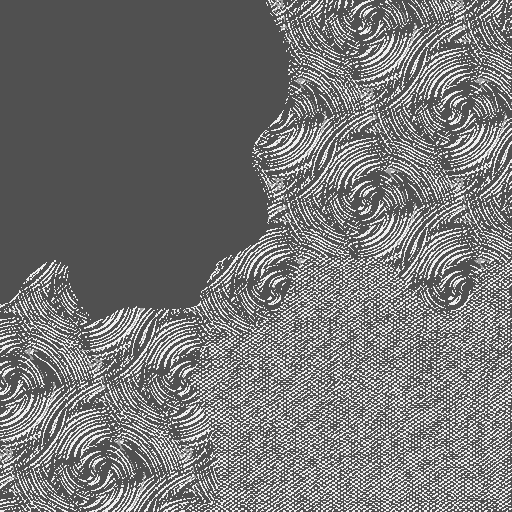
\includegraphics[width=\textwidth]{img/KMEANS.png}
                \caption{$KMEANS$}
            \end{subfigure}
            ~
            \begin{subfigure}[b]{0.3\textwidth}
                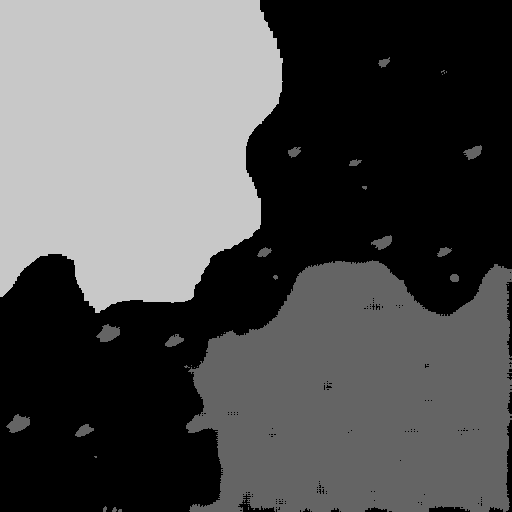
\includegraphics[width=\textwidth]{img/noiseK.png}
                \caption{$noiseK$}
            \end{subfigure}
            ~
            \begin{subfigure}[b]{0.3\textwidth}
                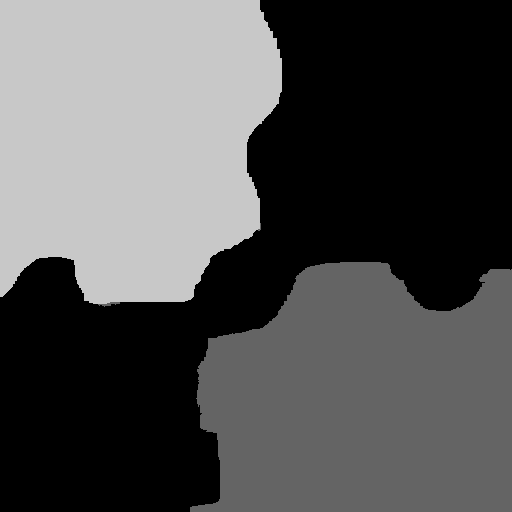
\includegraphics[width=\textwidth]{img/K.png}
                \caption{K.raw}
            \end{subfigure}

            \caption{Texture Analysis}
        \end{figure}

        \newpage
        \item Based on $K$, try to generate another texture image by exchange the types of different texture patterns.

        To exchange texture patterns, we first extract a $128 \times 128$ area for each texture patterns. Then we repeat each pattern for 16 times to get a full size $512 \times 512$ texture map.

        \begin{figure}[!htb]
            \centering
            \begin{subfigure}[b]{0.3\textwidth}
                
\includegraphics[width=\textwidth]{img/map1.png}
                \caption{$map1$}
            \end{subfigure}
            ~
            \begin{subfigure}[b]{0.3\textwidth}
                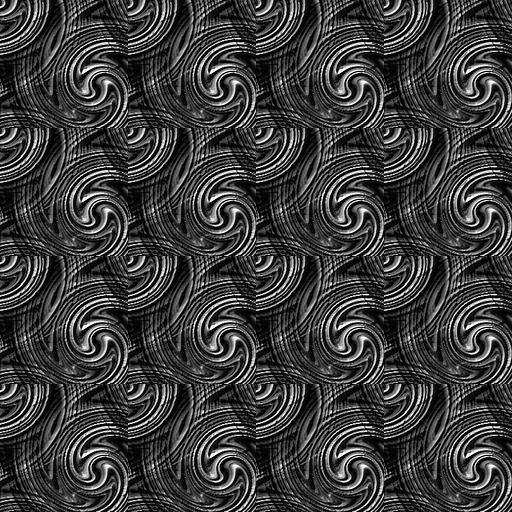
\includegraphics[width=\textwidth]{img/map2.png}
                \caption{$map2$}
            \end{subfigure}
            ~
            \begin{subfigure}[b]{0.3\textwidth}
                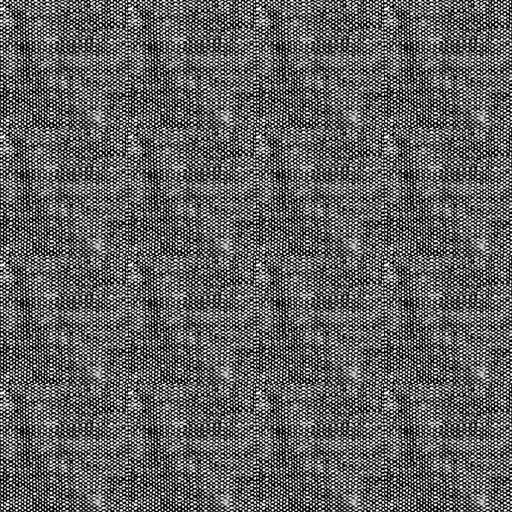
\includegraphics[width=\textwidth]{img/map3.png}
                \caption{$map3$}
            \end{subfigure}
        
            \caption{3 different texture maps}
        \end{figure} 

        For each entry in the $K$, there are three cases:

        \begin{enumerate}[label=(\roman*)]
            \item intensity = 0, change it to the corresponding entries of $map3$.
            \item intensity = 100, change it to the corresponding entries of $map1$.
            \item intensity = 200, change it to the corresponding entries of $map2$.
        \end{enumerate}

        \begin{figure}[!htb]
            \centering
            \begin{subfigure}[b]{0.3\textwidth}
                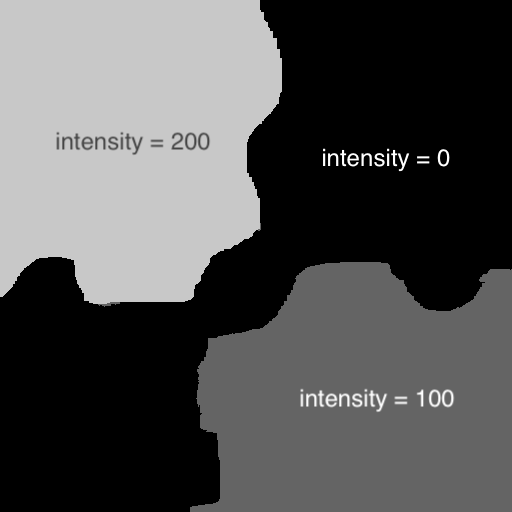
\includegraphics[width=\textwidth]{img/KI.png}
                \caption{$K$ with labeld intensities}
            \end{subfigure}
            ~
            \begin{subfigure}[b]{0.3\textwidth}
                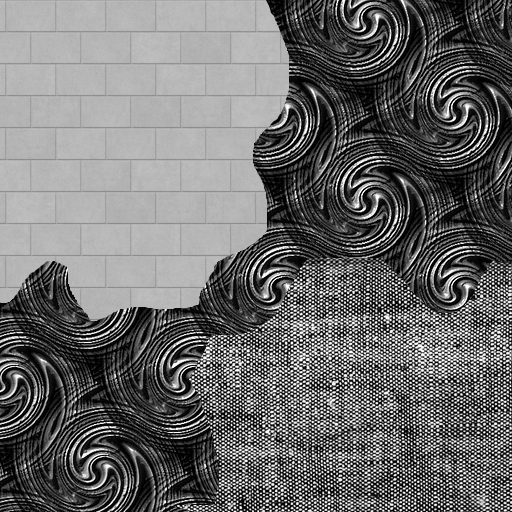
\includegraphics[width=\textwidth]{img/I2.png}
                \caption{$I_2$}
            \end{subfigure}
            ~
            \begin{subfigure}[b]{0.3\textwidth}
                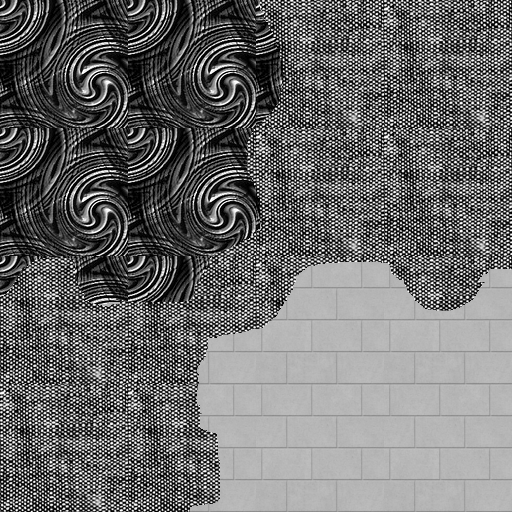
\includegraphics[width=\textwidth]{img/exchanged.png}
                \caption{$exchanged$}
            \end{subfigure}

            \caption{Texture Exchanging}
        \end{figure}   
    \end{enumerate}
\newpage
\subsection*{BONUS}
Given an image $I_3$ shown in Fig. 3, please try to produce an image as illustrated in Fig. 4 by adopting appropriate morphological processing. Please describe the designed algorithm in detail and provide some discussions. \\

I first apply Cross Median Filter with $window.size = 25$, thne use dilation method with $window.size = 11$ to enhance the given image.

\begin{figure}[!htb]
    \centering
    \begin{subfigure}[b]{0.3\textwidth}
        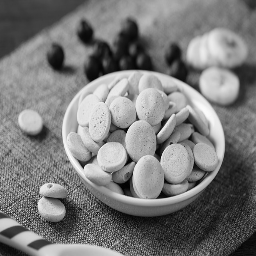
\includegraphics[width=\textwidth]{img/I3.png}
        \caption{I3.raw}
    \end{subfigure}
    ~
    \begin{subfigure}[b]{0.3\textwidth}
        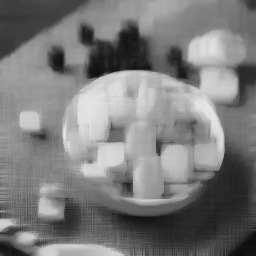
\includegraphics[width=\textwidth]{img/RS.png}
        \caption{$crossMedianFilter(I_3, 25)$}
    \end{subfigure}
    ~
    \begin{subfigure}[b]{0.3\textwidth}
        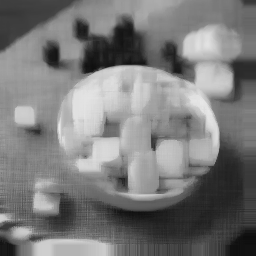
\includegraphics[width=\textwidth]{img/Dilated2.png}
        \caption{Blurred image}
    \end{subfigure}

    \caption{Blurred Image}
\end{figure}

\end{document}